%%%%%%%%%%%%%%%%%%%%%%%%%%%%%%%%%%%%%%%%%%%%%%%%%%%%%%%%%%%%%%%%%%%%%
%% This is a (brief) model paper using the achemso class
%% The document class accepts keyval options, which should include
%% the target journal and optionally the manuscript type. 
%%%%%%%%%%%%%%%%%%%%%%%%%%%%%%%%%%%%%%%%%%%%%%%%%%%%%%%%%%%%%%%%%%%%%
\documentclass[journal=jacsat,manuscript=article]{achemso}
\SectionNumbersOn
%\usepackage[letterpaper,left=0.5in,right=0.5in,top=1.0in,bottom=1.0in]{geometry}

%%%%%%%%%%%%%%%%%%%%%%%%%%%%%%%%%%%%%%%%%%%%%%%%%%%%%%%%%%%%%%%%%%%%%
%% Place any additional packages needed here.  Only include packages
%% which are essential, to avoid problems later. Do NOT use any
%% packages which require e-TeX (for example etoolbox): the e-TeX
%% extensions are not currently available on the ACS conversion
%% servers. 
%%%%%%%%%%%%%%%%%%%%%%%%%%%%%%%%%%%%%%%%%%%%%%%%%%%%%%%%%%%%%%%%%%%%%
\usepackage[version=3]{mhchem} % Formula subscripts using \ce{}
\usepackage{siunitx} % generating degrees Celsius in the document 
\usepackage{color}
\usepackage{soul} % allows highlighting text 
\usepackage{makecell}
\usepackage{booktabs}
\usepackage{amsmath}
\usepackage{amssymb}
\usepackage{todonotes}
\usepackage{gensymb}
\usepackage{verbatim}
\usepackage{hyperref}
\hypersetup{
    colorlinks=true,
    citecolor= red,
    linkcolor=blue,
    urlcolor=blue, 
    breaklinks=true
}
\usepackage{ulem}
\usepackage{float}


%%%%%%%%%%%%%%%%%%%%%%%%%%%%%%%%%%%%%%%%%%%%%%%%%%%%%%%%%%%%%%%%%%%%%
%% If issues arise when submitting your manuscript, you may want to
%% un-comment the next line.  This provides information on the
%% version of every file you have used.
%%%%%%%%%%%%%%%%%%%%%%%%%%%%%%%%%%%%%%%%%%%%%%%%%%%%%%%%%%%%%%%%%%%%%
%%\listfiles

%%%%%%%%%%%%%%%%%%%%%%%%%%%%%%%%%%%%%%%%%%%%%%%%%%%%%%%%%%%%%%%%%%%%%
%% Place any additional macros here.  Please use \newcommand* where
%% possible, and avoid layout-changing macros (which are not used
%% when typesetting).
%%%%%%%%%%%%%%%%%%%%%%%%%%%%%%%%%%%%%%%%%%%%%%%%%%%%%%%%%%%%%%%%%%%%%
\newcommand*\mycommand[1]{\texttt{\emph{#1}}}
\DeclareRobustCommand
  \Compactcdots{\mathinner{\cdotp\mkern-2mu\cdotp\mkern-2mu\cdotp}}

%%%%%%%%%%%%%%%%%%%%%%%%%%%%%%%%%%%%%%%%%%%%%%%%%%%%%%%%%%%%%%%%%%%%%
%% Meta-data block
%% ---------------
%% Each author should be given as a separate \author command.
%%
%% Corresponding authors should have an e-mail given after the author
%% name as an \email command. Phone and fax numbers can be given
%% using \phone and \fax, respectively; this information is optional.
%%
%% The affiliation of authors is given after the authors; each
%% \affiliation command applies to all preceding authors not already
%% assigned an affiliation.
%%
%% The affiliation takes an option argument for the short name.  This
%% will typically be something like "University of Somewhere".
%%
%% The \altaffiliation macro should be used for new address, etc.
%% On the other hand, \alsoaffiliation is used on a per author basis
%% when authors are associated with multiple institutions.
%%%%%%%%%%%%%%%%%%%%%%%%%%%%%%%%%%%%%%%%%%%%%%%%%%%%%%%%%%%%%%%%%%%%%
\author{Stephen P. Vicchio}
\affiliation[Clemson University]
{Department of Chemical and Biomolecular Engineering, Clemson University, Clemson, SC}
\author{Zhihengyu Chen}
\affiliation[Stony Brook University]
{Department of Chemistry, Stony Brook University, Stony Brook, NY}
\author{Karena Chapman}
\email{karena.chapman@stonybrook.edu}
\affiliation[Stony Brook University]
{Department of Chemistry, Stony Brook University, Stony Brook, NY}
\author{Rachel B. Getman}
\email{rgetman@clemson.edu}
\affiliation[Clemson University]
{Department of Chemical and Biomolecular Engineering, Clemson University, Clemson, SC}

%%%%%%%%%%%%%%%%%%%%%%%%%%%%%%%%%%%%%%%%%%%%%%%%%%%%%%%%%%%%%%%%%%%%%
%% The document title should be given as usual. Some journals require
%% a running title from the author: this should be supplied as an
%% optional argument to \title.
%%%%%%%%%%%%%%%%%%%%%%%%%%%%%%%%%%%%%%%%%%%%%%%%%%%%%%%%%%%%%%%%%%%%%
\title[manuscript]{
Understanding the ligand environment of a four ion \ce{Ni} cluster supported on the NU-1000 Metal-Organic Framework 
}

%%%%%%%%%%%%%%%%%%%%%%%%%%%%%%%%%%%%%%%%%%%%%%%%%%%%%%%%%%%%%%%%%%%%%
%% Some journals require a list of abbreviations or keywords to be
%% supplied. These should be set up here, and will be printed after
%% the title and author information, if needed.
%%%%%%%%%%%%%%%%%%%%%%%%%%%%%%%%%%%%%%%%%%%%%%%%%%%%%%%%%%%%%%%%%%%%%
\abbreviations{IR,NMR,UV}
\keywords{American Chemical Society, \LaTeX}

%%%%%%%%%%%%%%%%%%%%%%%%%%%%%%%%%%%%%%%%%%%%%%%%%%%%%%%%%%%%%%%%%%%%%
%% The manuscript does not need to include \maketitle, which is
%% executed automatically.
%%%%%%%%%%%%%%%%%%%%%%%%%%%%%%%%%%%%%%%%%%%%%%%%%%%%%%%%%%%%%%%%%%%%%
\begin{document}

%%%%%%%%%%%%%%%%%%%%%%%%%%%%%%%%%%%%%%%%%%%%%%%%%%%%%%%%%%%%%%%%%%%%%
%% The "tocentry" environment can be used to create an entry for the
%% graphical table of contents. It is given here as some journals
%% require that it is printed as part of the abstract page. It will
%% be automatically moved as appropriate.
%%%%%%%%%%%%%%%%%%%%%%%%%%%%%%%%%%%%%%%%%%%%%%%%%%%%%%%%%%%%%%%%%%%%%
%\begin{tocentry}
%
%Some journals require a graphical entry for the Table of Contents.
%This should be laid out ``print ready'' so that the sizing of the
%text is correct.
%
%Inside the \texttt{tocentry} environment, the font used is %Helvetica
%8\,pt, as required by \emph{Journal of the American Chemical
%Society}.
%
%The surrounding frame is 9\,cm by 3.5\,cm, which is the maximum
%permitted for  \emph{Journal of the American Chemical Society}
%graphical table of content entries. The box will not resize if the
%content is too big: instead it will overflow the edge of the box.
%
%This box and the associated title will always be printed on a
%separate page at the end of the document.
%
%\end{tocentry}

%%%%%%%%%%%%%%%%%%%%%%%%%%%%%%%%%%%%%%%%%%%%%%%%%%%%%%%%%%%%%%%%%%%%%
%% The abstract environment will automatically gobble the contents
%% if an abstract is not used by the target journal.
%%%%%%%%%%%%%%%%%%%%%%%%%%%%%%%%%%%%%%%%%%%%%%%%%%%%%%%%%%%%%%%%%%%%%
\begin{abstract}
Heterogeneous catalysts exhibit dynamic changes in composition and structure as a function of operating conditions that have a profound effect on catalytic performance. For traditional bulk metal heterogeneous catalysts, general trends between composition/structure and function are well established. However, single-site heterogeneous catalysts (SSHCs) where the active site consists of small metal clusters anchored to a solid support the same trends remain undefined. One such SSHC involves a 3d transition metal complex (i.e., \ce{Ni_4O_xH_y}) supported on a porous metal-organic framework (MOF). Herein, we investigate the ligand environment of a \ce{Ni4} cluster supported on the NU-1000 MOF when exposed to reducing conditions (\ce{H2} gas), with the ligand environment varying from \ce{O}, \ce{OH}, \ce{H2O}, and \ce{H} ligands coordinated to the \ce{Ni} atoms. Differential pair distribution functions (d-PDF) analysis and \textit{ab initio} thermodynamic analysis probe potential ligand environments of the \ce{Ni_4O_xH_y} cluster. We generate over 300 different structures featuring different \ce{Ni4} clusters (i.e., different ligand environments) while also accounting for the spin states of the \ce{Ni} atoms. Phase diagrams show the relative location of thermodynamically relevant conditions as a function of \ce{H2} and \ce{H2O} chemical potential terms, and d-PDF analysis enables comparisons in local structural information to experimental data. Structures with \ce{Ni-O} coordination numbers closer to experimental data occur at high \ce{H2O} chemical potentials, suggesting a large \ce{H2O} chemical potential is present within the MOF. Reasonable agreement is seen in the \ce{Ni-O} peak between model and experimental d-PDFs; however, model structures fail to recreate the split \ce{Ni{\Compactcdots}Ni} peaks. Furthermore, d-PDF analysis suggests that asymmetric ligand environments in structures containing high \ce{Ni-O} coordination demonstrate features that are most closely related to the experimental structure, such as the \ce{Ni-O} peak and the split \ce{Ni{\Compactcdots}Ni} peaks. The combined modeling approach demonstrates how the SSHC active site structure is sensitive to the environment conditions, and provide insights into the correct coordination environment of the \ce{Ni4} cluster supported on the NU-1000 MOF thereby establish general trends in the \ce{Ni} ligand environment for these heterogeneous catalytic systems.

\end{abstract}

%%%%%%%%%%%%%%%%%%%%%%%%%%%%%%%%%%%%%%%%%%%%%%%%%%%%%%%%%%%%%%%%%%%%%
%% Start the main part of the manuscript here.
%%%%%%%%%%%%%%%%%%%%%%%%%%%%%%%%%%%%%%%%%%%%%%%%%%%%%%%%%%%%%%%%%%%%%

\section{Introduction}
%%%%%%%%%%%%%%%%%%%%%%%%%%%%%%%%%%%%%%%%%%%%%%%%%%%%%%%%%%%%%%%%%%%%%
%% Introduction
%%%%%%%%%%%%%%%%%%%%%%%%%%%%%%%%%%%%%%%%%%%%%%%%%%%%%%%%%%%%%%%%%%%%%

Single-site heterogeneous catalysts (SSHCs) contain well-defined, atomically dispersed active sites that are anchored to solid supports,\cite{Hlatky2000, Kaiser2020, Wasson2019} such as metal-organic frameworks (MOFs),\cite{Zheng2019, AbdelMageed2019, Huang2019} covalent-organic frameworks (COFs),\cite{Zhong2019, Romero-Muniz2020} zeolites,\cite{Mao2016, Kistler2014} and metal\cite{Patel2019, Pei2017, Jiao2019} and metal oxide surfaces.\cite{Bo2019, Riley2018, Tang2019} The atomically dispersed atoms are often 3d transition metals,\cite{Manna2016, Beyzavi2015} with the solid support providing a means to improve metal utilization and maintain well-defined active site structures.\cite{Qiao2011, Cui2017, Yang2013} The metal atoms are anchored to the support either directly (metal-metal bonds) or by organic ligands (e.g., \ce{OH}-ligands), with the attachment dependent on the type of support. In some cases, the ligand environments may be similar to homogeneous catalysts.\cite{Rogge2017} Also similar to homogeneous catalysts, active site structures for SSHCs can be tuned by changing the ligand environment and metal atoms. SSHCs are hence appealing for carrying out challenging chemistries.\cite{Thomas2005, Liu2019, Desai2018}

For SSHCs, the structural environments (i.e, the coordinate ligands) of the metal atom centers drive the catalysis.\cite{DeRita2019} However, predicting the ligand environment of any SSHC is non-trivial due to the uniqueness of active site,\cite{Daelman2019, Tang2019} and is further complicated by structural changes induced by operating conditions.\cite{Li2018, Kim2015} Understanding the SSHC ligand environment is imperative to understand the catalytic mechanisms that occur. Difficulties in determining the precise active site for SSHCs remain an ongoing challenge, with a lack of structural information about the active site preventing detailed structures-function relationships between catalyst structure and performance.

In this work, we seek to learn the composition and structure of a \ce{Ni} SSHC under conditions relevant to catalytic hydrogenation. \ce{Ni}-based catalysts are important in a variety of reactions, including ethene oligomerization using the Shell higher oligomers process (SHOP)\cite{1988Reuben} and the steam reforming of methane using the Catalytic Rich Gas (CRG) catalyst.\cite{Ross1973} Specifically, we investigate a \ce{Ni} cluster supported on the MOF NU-1000, herein denoted Ni-NU-1000. MOFs are porous crystals that consist of metal cation nodes connected by organic ``linker" molecules.\cite{Li1999} NU-1000 (Figure~\ref{fig:Ni-MOF-model}a) is comprised of \ce{Zr6(\mu_{3}-O)4(\mu_{3}-OH)4(H2O)4(OH)4} nodes interconnected with tetratopic 1,3,6,8-tetrakis (p-benzoate) pyrene (TBAPy) linkers. The \ce{Ni} ions are known to anchor to the NU-1000 nodes via the accessible \ce{-OH}/\ce{-OH2} ligands on the \ce{Zr6} nodes, with Atomic Layer Deposition in MOFs (AIM) depositing the \ce{Ni} atoms.\cite{Mondloch2013} Initially, the structure was thought to consist of a single divalent \ce{Ni} ion coordinated with zero to three \ce{H2O} ligands, depending on the operating conditions.\cite{Li2016sintering} However, difference envelope density (DED) analysis of powder diffraction data and electron microscopy later revealed that the catalyst is four \ce{Ni} ion cluster (\ce{Ni4O_{x}H_{y}}) and contains a combination of hydroxo (\ce{OH}) and water \ce{H2O} ligands.\cite{PlateroPrats2017} Additional computational studies by \citeauthor{Ye2017} then suggested the four \ce{Ni} ion cluster is attached to adjacent nodes within Ni-NU-1000.\cite{Ye2017} Key questions remain about the precise ligand environment of the \ce{Ni} ions. Prior literature for Ni-NU-1000 suggests that the \ce{Ni} ions are interconnected by \ce{OH}-ligands and are coordinated by \ce{H2O}-ligands; however, the precise ligand environment (i.e., the composition and arrangement of the ligands) isn't fully established. Additionally, several modeling studies for catalytic ethylene hydrogenation\cite{Li2016sintering, Shabbir2020} and dimerization\cite{Ye2017} in Ni-NU-1000 utilize a \ce{Ni} hydride (\ce{Ni-H}) active site model, which \citeauthor{Yeh2021} determined is the preferred active site model for a \ce{Ni} ion cluster supported on the UiO-66 MOF (rather than NU-1000).\cite{Yeh2021} Addressing questions related to the active site structure are important in improving these Ni-NU-1000 catalysts, and the results will be useful for understanding ligand environments in other 3d transition metal ion catalysts as well.   

Along these lines, in this work, we explore the ligand environment of a four ion \ce{Ni} cluster under conditions relevant to catalytic hydrogenation (specifically conditions with exposure to \ce{H2} gas during the activation step). Prior experimental work on Ni-NU-1000 enables comparisons between computational and experimental characterization. We combine differential pair distribution function (d-PDF) analysis, density functional theory (DFT), and \textit{ab initio} thermodynamic modeling to learn the ligand environment of Ni-NU-1000. We find that highly coordinated \ce{Ni} ions (\ce{Ni-O} coordination $\sim$5) that contain an asymmetric arrangement of \ce{OH}, \ce{H2O}, and \ce{O} ligands show the best agreement with experimental results. Structures that can achieve such high \ce{Ni} coordination exhibit large chemical potentials of \ce{H2O} even under reducing conditions, suggesting that NU-1000 is able to store \ce{H2O} under these conditions. Notably, we only identify one structure featuring a \ce{Ni} hydride in thermodynamic modeling, despite the the consensus that metal (M) hydrides are part of the active site in M-NU-1000 catalysts. Our results provide insights into the local coordination of the \ce{Ni} metal cluster that will be useful in hypothesizing and modeling catalytic mechanisms on such catalysts. 

\begin{figure}
    \centering
    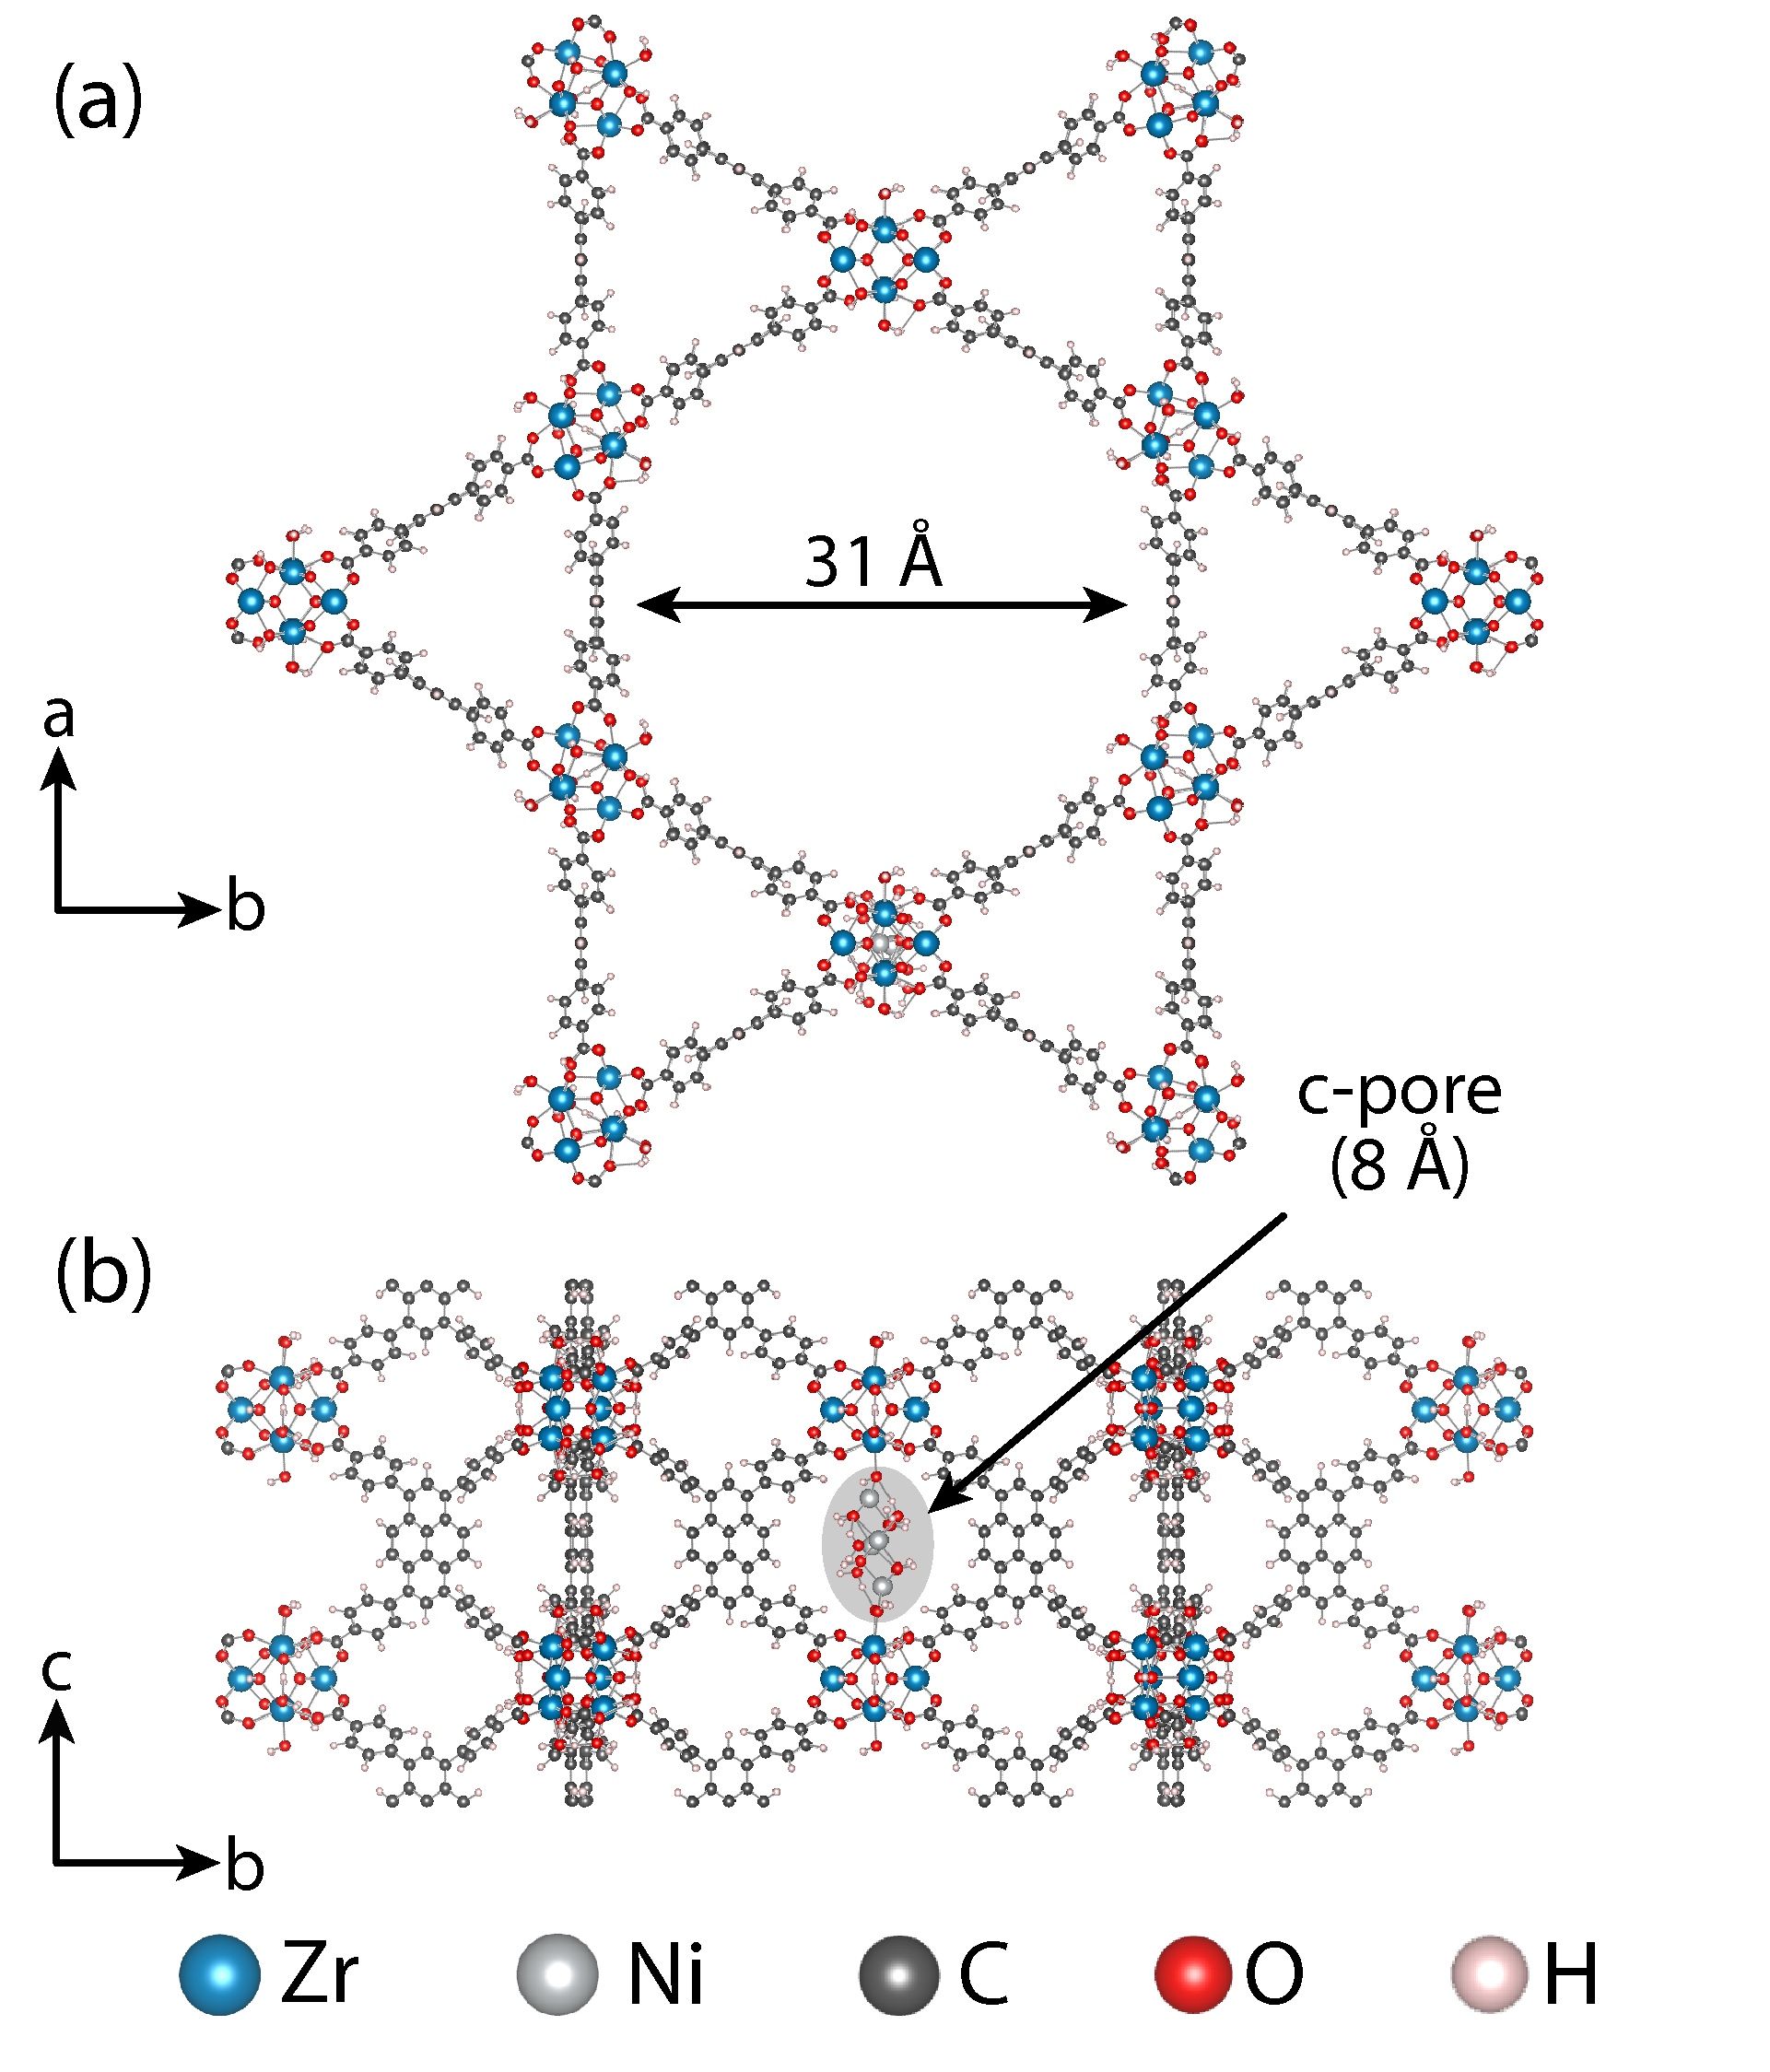
\includegraphics[width=3.0in]{zi-images/00-General-Graphics/2022-figure-MOF-schematic.png}
    \caption{
    The structure of NU-1000 shown along the (a) c-axis and the (b) a-axis with the location of the \ce{Ni} metal cluster highlighted by the gray oval. The metal cluster is located within the 8~{\AA} pore of Ni-NU-1000. The diameters of the hexagonal (31~{\AA}) and triangular (10~{\AA}) channels are also indicated.
    }
    \label{fig:Ni-MOF-model}
\end{figure}

\section{Methodology}
%%%%%%%%%%%%%%%%%%%%%%%%%%%%%%%%%%%%%%%%%%%%%%%%%%%%%%%%%%%%%%%%%%%%%
%% Methodology
%%%%%%%%%%%%%%%%%%%%%%%%%%%%%%%%%%%%%%%%%%%%%%%%%%%%%%%%%%%%%%%%%%%%%

\subsection{Differential Pair Distribution Function Analysis}

Differential pair distribution function (d-PDF) analysis is performed to reveal key interatomic distances in the Ni-NU-1000 catalysts and provide insight into the structure and ligand environment. Ni-NU-1000 catalysts are synthesized using AIM as described previously.\cite{Mondloch2013, Li2016sintering} Synthesized catalysts are then exposed to \ce{H2} (3.5\% in \ce{He}) at 200 \degree C for 2 hours and then cooled to 50 \degree C in \ce{H2}.\cite{PlateroPrats2017} Powder X-ray diffraction (XRD) and total scattering data suitable for PDF analysis are then collected at 50 \degree C in \ce{H2}. PDFs are then taken using the PDFgui software;\cite{Farrow2007} details of these simulations are described in detail elsewhere.\cite{PlateroPrats2017}. PDFs represent the local structure as a histogram of atom-atom distances in the material weighted by the scattering power of the atoms involved. These are used to derive d-PDFs by subtracting the PDF measured for NU-1000 from the PDF measured for Ni-NU-1000, to isolate the atom-atom distances that define the \ce{Ni} cluster and its interaction with NU-1000 support. Of interest are the \ce{Ni{\Compactcdots}Ni}, \ce{Ni-O}, and \ce{O{\Compactcdots}O} distances within the cluster and the \ce{Ni{\Compactcdots}Zr} and \ce{Ni{\Compactcdots}O} distances between the cluster and NU-1000. In this notation, atom pairs not directly bonded to each other are denoted with ``${\Compactcdots}$". Given the lower scattering contribution from the \ce{O} atoms compared to \ce{Ni} atoms, \ce{O{\Compactcdots}O} pairs have very low contribution to the measured data and are not calculated. PDFs of the computed structural models are simulated using typical values of instrument and atomic displacement parameters for such materials and then evaluated for their correspondence to the experimental data over XYZ {\AA} range.  

\subsection{Computational Details}

\subsubsection{Catalyst Structure Models}

NU-1000 (P6/mmm space group) features small 8~{\AA} pores with uniform hexagonal (31~{\AA}) and triangular (10~{\AA}) channels (Figure \ref{fig:Ni-MOF-model}). DFT-optimized unit cell parameters are $a=b=40.611$ {\AA}, $c=15.990$ {\AA}, $\alpha=\beta=\ang{90}$, and $\gamma=\ang{60}$. Simulated structures contain one \ce{Ni} cluster per unit cell. Based on the current knowledge about Ni-NU-1000 catalysts,\cite{PlateroPrats2017} these clusters comprise four \ce{Ni} ions and span the small pores of NU-1000, connecting two adjacent nodes (Figure~\ref{fig:Ni-MOF-model}b). (Structures comprising fewer than four \ce{Ni} ions were also evaluated, but gave poor agreement with the experimental d-PDF; see \hl{Supporting Information Section XXX}.) Clusters bind to the nodes by replacing two protons (one on each node).\cite{Ye2017} To provide molecular-level insight into the types of ligand environments that could lead to the experimentally observed d-PDFs, we consider \hl{854} different structures comprising a variety of ligand environments, including hydroxyl (\ce{OH}), water (\ce{H2O}), hydride (\ce{H}), and oxygen (\ce{O}), giving stoichiometries of \ce{Ni_4O_xH_y} for all clusters considered. Four example structures are shown in Figure~\ref{fig:Ni-MOF-structures}. The full library of structures considered in this work can be accessed on our GitHub page.\cite{GitHub-Ni4Project}

\begin{figure}
    \centering
    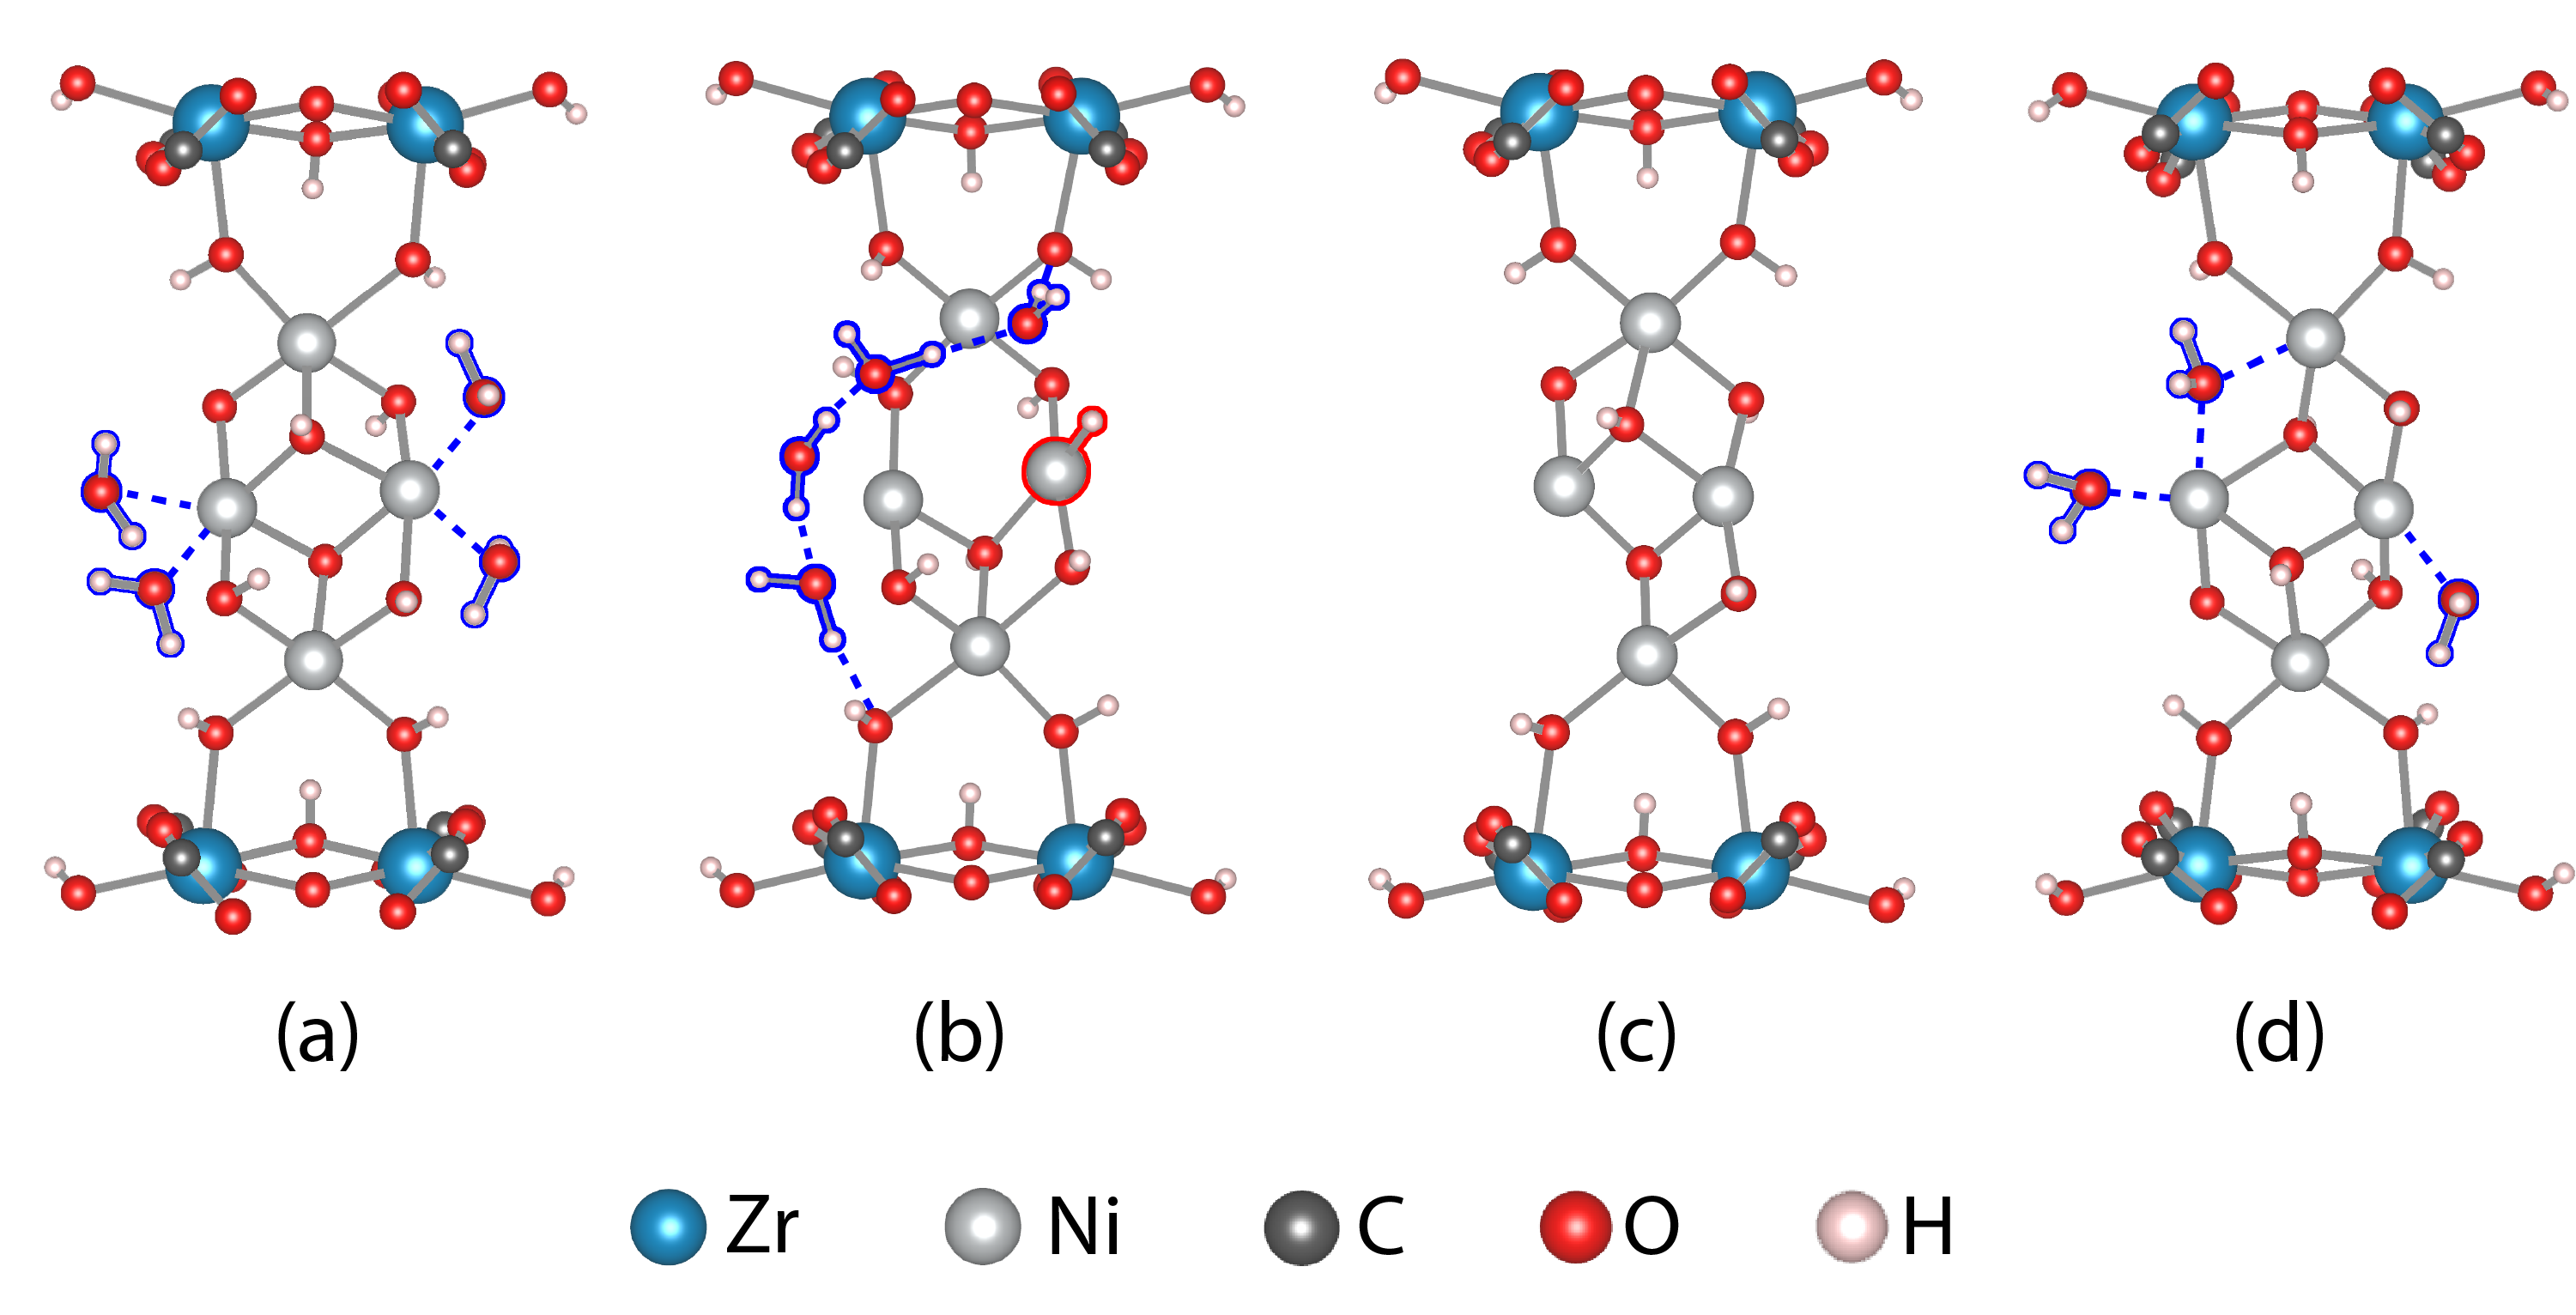
\includegraphics[width=5.0in]{zi-images/00-General-Graphics/2022-figure-clusters-3xstructures.png}
    \caption{
    Some of the \ce{Ni_4O_xH_y} clusters evaluated in this work. (a) \ce{Ni4(OH)6.4H2O} (green), (b) \ce{Ni4(OH)5(H).4H2O} (blue), (c) \ce{Ni4(OH)4(O)} (yellow), and (d) \ce{Ni4(OH)4(O).3H2O} (maroon). Colors in parentheses are the same as for Figures~\ref{fig:phase_diagram_Ni} and \ref{fig:Ni-structure-diagram}. The NU-1000 structure is excluded from the pictures for clarity, except for the \ce{Zr} ions where the clusters are attached. The atom color key is indicated in the figure. \ce{H2O} molecules and ligands are outlined in blue, and \ce{Ni-H} ligands are outlined in red.
    }
    \label{fig:Ni-MOF-structures}
\end{figure}

\subsubsection{\textit{ab initio} Thermodynamics Modeling}

\textit{ab initio} thermodynamic analysis\cite{Reuter2003, Reuter2004, Grundner2015, Paolucci2016, Li2016, Getman2008, Mandal2020, Zuo2016, Tang2019} is used to determine the thermodynamically stable structures as functions of chemical potential (which can be related to gas phase temperature and partial pressure using an equation of state; \hl{see Supporting Information} Section \hl{XXX}). We specifically consider chemical potentials of \ce{H2} (g) ($\mu_{\ce{H2}}$) and \ce{H2O} (g) ($\mu_{\ce{H2O}}$). \ce{H2} (g) is chosen since experimental d-PDFs were collected under hydrogenation conditions. \ce{H2O} (g) is chosen since we find hydrogen atom binding on the cluster often occurs on hydroxyl ligands, forming \ce{H2O} ligands, which can then desorb. \ce{H2O} (g) is hence a convenient oxygen reference.  Cluster free energies are then calculated as:
\begin{equation}
    \begin{split}
        \Delta F^{(2)}(V,T,\mu_{\text{H}},\mu_{\text{O}},N_{\text{Ni}})  
        & = \Delta F(V,T,N_{\text{H}},N_{\text{O}},N_{\text{Ni}}) - (\mu_{\text{H}})(\Delta N_{\text{H}}) \\
        & - (\mu_{\text{O}})(\Delta N_{\text{O}})  \\ 
    \end{split}
    \label{eq:free-energy-trans}
\end{equation}
where $F^{(2)}$ is the the second Legendre transform of the Helmholtz free energy (i.e., of $N_{\ce{H}}$ and $N_{\ce{O}}$ to $\mu_{\ce{H}}$ and $\mu_{\ce{O}}$),\cite{Alberty1997} $V$ is volume, $T$ is temperature, $\mu$ is chemical potential, and $N$ is number, i.e., of \ce{O} and \ce{H} atoms within the cluster. $\mu_{\ce{H}} = \frac{1}{2} \mu_{\ce{H}_2}$, and $\mu_{\text{O}} = \mu_{\ce{H2O}} - 2\mu_{\ce{H}}$. $F = E^\text{elec} + E^\text{ZP} + F^\text{vib}$, where $E^\text{elec}$ is the electronic energy calculated with DFT, $E^\text{ZP}$ is the zero point vibrational energy, and $F^\text{vib}$ is the temperature dependent vibrational free energy. The $\Delta$'s in Eq.~\ref{eq:free-energy-trans} indicate quantities taken relative to a reference structure; the reference structure used in this work is shown in Figure~\ref{fig:Ni-MOF-structures}a. This structure comprises \ce{OH} and \ce{H2O} ligands (outlined in blue in Figure~\ref{fig:Ni-MOF-structures}) and is highly symmetric.

\subsubsection{Density Functional Theory Calculations}
Electronic energies are calculated using the CP2K software package\cite{Hutter2014} using the PBE exchange and correlation functional\cite{Perdew1996}, damped D3 dispersion corrections,\cite{Grimme2010} the DZVP-MOLOPT basis set,\cite{VandeVondele2007} and Goedecker pseudopotentials.\cite{Goedecker1996} Plane waves are simulated up to 360 Ry. As a single divalent \ce{Ni} ion can adopt singlet or triplet spin states, we evaluate singlet, triplet, quintet, septet, and nonet states for the \ce{Ni4} clusters, following prior work.\cite{Shabbir2020, Ye2017, Bernales2016} The Unrestricted Kohn-Sham (UKS) method is employed given the open shell nature of the system. Spin states exhibiting spin contamination are not considered in \textit{ab initio} thermodynamic analysis. Details about how spin contamination is determined and the criteria used to keep or discard structures is provided in Supporting Information Section \hl{XXX}. Electronic energies are obtained from geometry relaxations where all atoms in the periodic unit cell are allowed to relax. $E^\text{ZP}$ and $F^\text{vib}$ are calculated from the calculated vibrational modes. Details about how the vibrational modes, $E^\text{ZP}$, and $F^\text{vib}$ are calculated are provided in \hl{Supporting Information}. Vibrational modes are only calculated for structures within 100 kJ/mol of the lowest electronic-energy cluster at each unique composition to decrease computational expense. Details about how $E_{\text{H}_2}$ and $E_{\text{H}_2\text{O}}$ are calculated and sample CP2K input files for all types of DFT calculations carried out in this work are provided in Supporting Information. 

\section{Results and Discussion}
%%%%%%%%%%%%%%%%%%%%%%%%%%%%%%%%%%%%%%%%%%%%%%%%%%%%%%%%%%%%%%%%%%%%%
%% Results 
%%%%%%%%%%%%%%%%%%%%%%%%%%%%%%%%%%%%%%%%%%%%%%%%%%%%%%%%%%%%%%%%%%%%%

% d-PDF Diagram
\begin{figure}
    \centering
    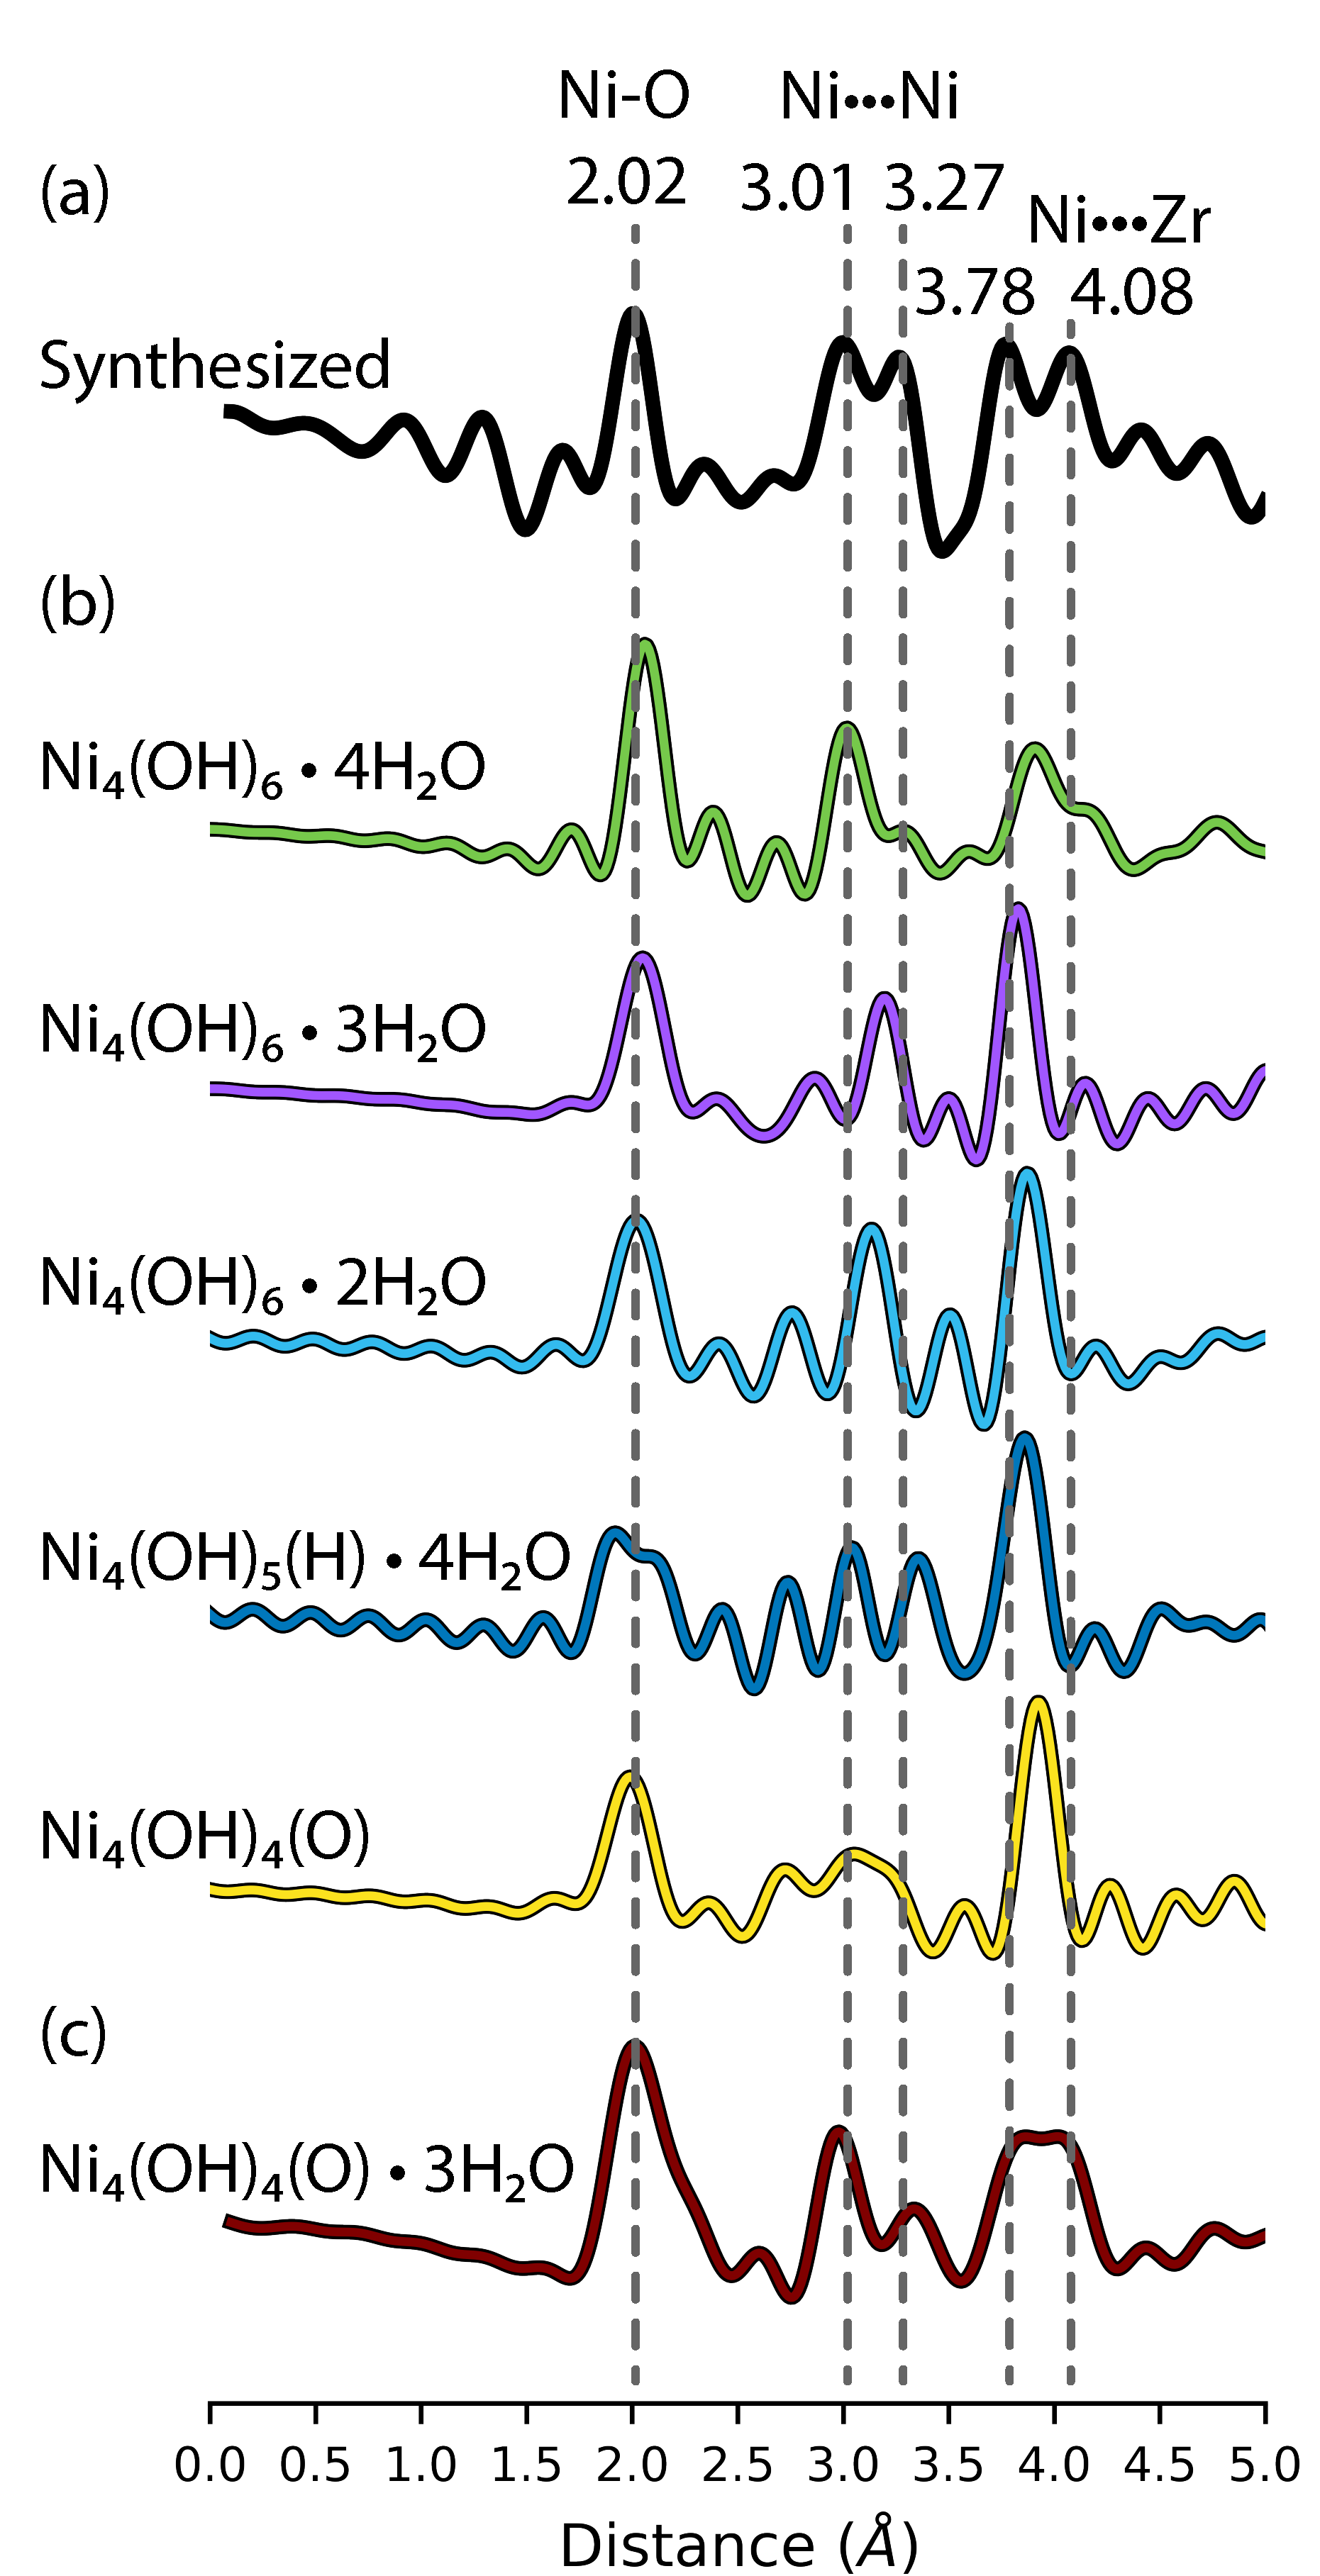
\includegraphics{zi-images/01-Ni-Graphics/2021-MAIN-single-dPDF.png}
    \caption{
    d-PDFs for (a) the synthesized structure, (b) simulated structures representing thermodynamic minima with \ce{Ni-O} coordination numbers $\ge$ 4, and (c) the simulated structure that gives the best agreement with the synthesized structure. Structure labels and colors for the simulated structures are the same as in the text and in Figures~\ref{fig:phase_diagram_Ni} and \ref{fig:Ni-structure-diagram}. Gray dotted lines indicate key distances observed for the synthesized structure, which are also annotated on the figure.
    }
    \label{fig:dPDFs-graphic}
\end{figure}

The d-PDF for the synthesized Ni-NU-1000 catalyst is shown in Figure~\ref{fig:dPDFs-graphic}a.\cite{PlateroPrats2017} Key peaks are the single peak at 2.02 {\AA}, split peaks at 3.01 {\AA} and 3.27 {\AA}, and split peaks at 3.78 {\AA} and 4.08 {\AA}, which correspond to \ce{Ni-O}, \ce{Ni{\Compactcdots}Ni}, and \ce{Ni{\Compactcdots}Zr} distances, respectively. Prior work indicates that the \ce{Ni-O} coordination number is $\sim$5.\cite{PlateroPrats2017} 

Figure~\ref{fig:phase_diagram_Ni} plots a phase diagram constructed using \textit{ab initio} thermodynamic analysis that indicates the thermodynamically most stable structures within the simulated database. In this phase diagram, the different colored regions correspond to different structures, which are depicted in Figure~\ref{fig:Ni-structure-diagram}. Each structure is annotated with its \ce{Ni-O} coordination number; ranges of $\mu_{\ce{H2}}$ and $\mu_{\ce{H2O}}$ are selected such that coordination numbers $\sim$5 are centered. (Expansion of the phase diagram to higher and lower values of $\mu_{\text{H}_2\text{O}}$ and $\mu_{\text{H}_2}$ does not reveal any additional structures or higher coordination numbers; See \hl{Supporting Information Section XX} for further details.) The structures \ce{Ni4(OH)6.2H2O} (cyan), \ce{Ni4(OH)6.3H2O} (purple), and \ce{Ni4(OH)6.4H2O} (green) give \ce{Ni-O} coordination numbers of 4.5, 5.0, and 5.5, which are in line with the experimentally observed value of $\sim$5. These structures comprise significant \ce{OH} and \ce{H2O} ligands and no \ce{O} or \ce{H} ligands and have stoichiometries of \ce{Ni4O8H10}, \ce{Ni4O9H12}, and \ce{Ni4O10H14}, respectively. They reside on the phase diagram at higher (more positive) values of $\mu_{\text{H}_2\text{O}}$ and lower (more negative) values of $\mu_{\text{H}_2}$. As these structures in agreement with the experimentally observed \ce{Ni-O} coordination number are stable at higher values of chemical potential, which correspond to larger concentrations (and lower temperatures), this finding suggests that NU-1000 comprises significant \ce{H2O} concentration, even after exposure to \ce{H2}/\ce{He} at 200 \degree C for 2 hours and measurement in \ce{H2}/\ce{He} at 50 \degree C. Similar \ce{H2O} storage properties have been observed in MOF-303\cite{Hanikel2021} and MOF-801\cite{Kim2017} under ambient conditions. The vertical dotted line in Figure~\ref{fig:Ni-structure-diagram} indicates values of $\mu_{\ce{H2}}$ used during collection of the experimental d-PDF. The structures \ce{Ni4(OH)6.3H2O} (purple) and \ce{Ni4(OH)6.4H2O} (green) fall along this line in Figure~\ref{fig:Ni-structure-diagram} and have significant \ce{OH} and \ce{H2O} content.        

% Phase Diagram
\begin{figure}[H]
    \centering
    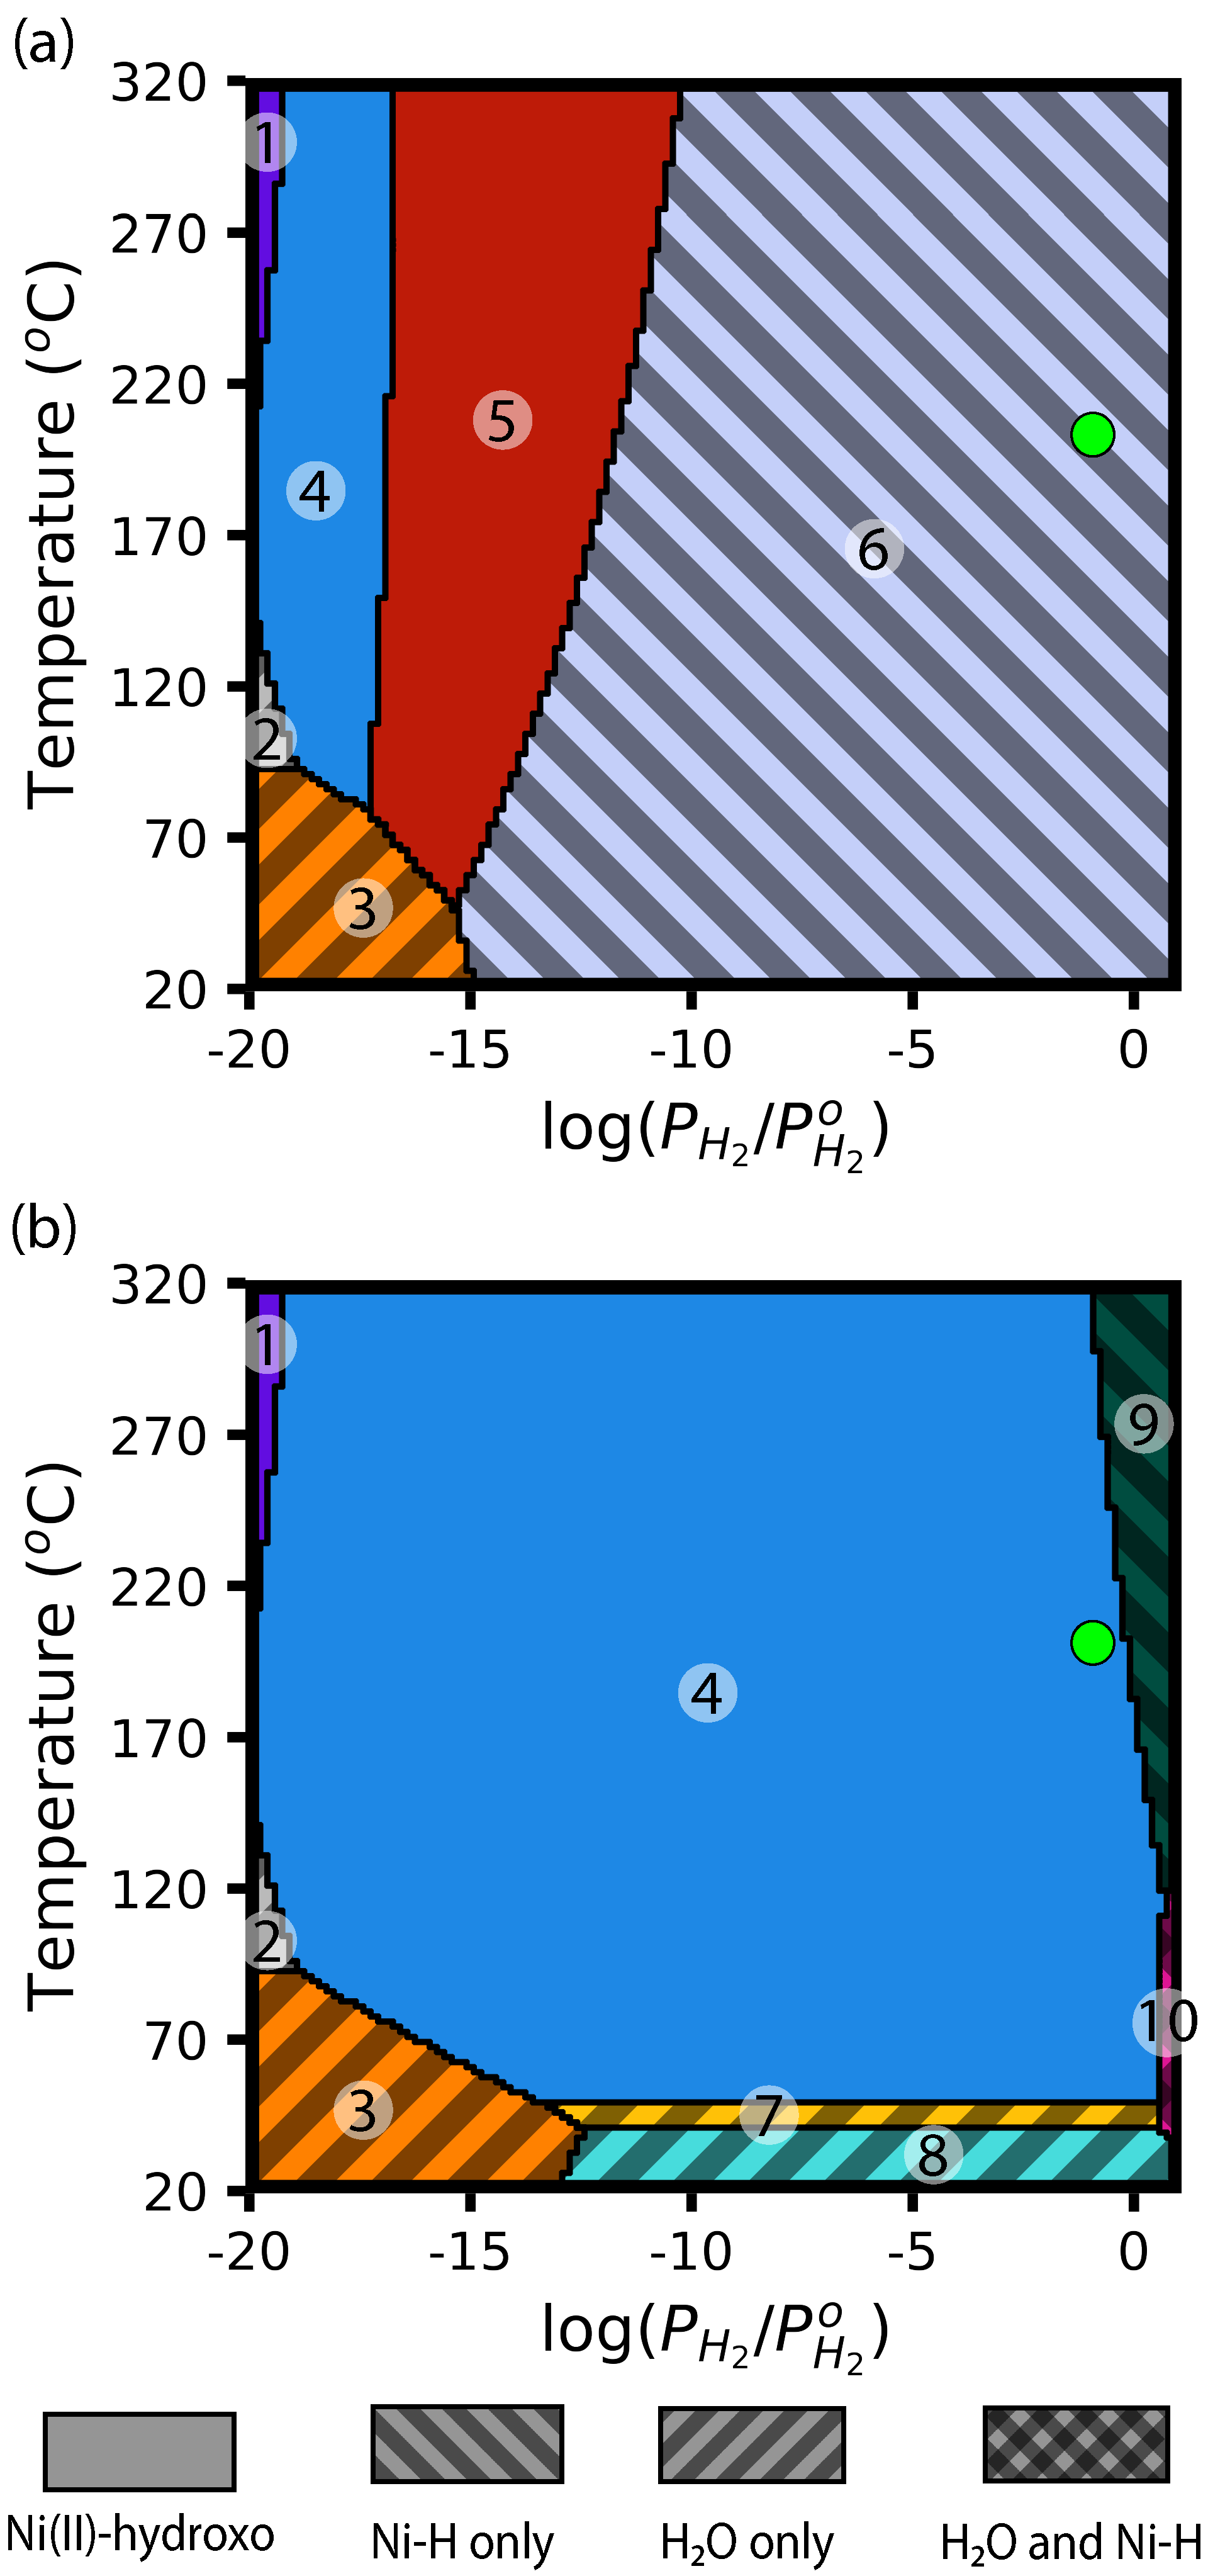
\includegraphics{zi-images/01-Ni-Graphics/2021-MAIN-phase-diagram-combined.png}
    \caption{
    Calculated phase diagram for the \ce{Ni4} cluster presented as a function of $\Delta \mu_{\ce{H2}}$ and $\Delta \mu_{\ce{H2O}}$, where the $\Delta$'s indicate the values are referenced to the 0~K values (derivation provided in Supporting Information). The different colored regions indicate different structures and follow the same key as in Figures~\ref{fig:dPDFs-graphic} and \ref{fig:Ni-structure-diagram}. The numbers indicate the \ce{Ni-O} coordination number. The hash patterns indicate the types of ligand environments and follow the key in the figure. The vertical dashed line indicates the value of $\Delta \mu_{\text{H}_2}$ corresponding to the conditions where the experimental d-PDF was collected (\ce{H2} in 3.5\% in \ce{He} at 50 \degree C and ambient pressure). As \ce{H2O} was not added in experiments, values of $\Delta \mu_{\ce{H2O}}$ are chosen such that the \ce{Ni-O} coordination number matches the experimentally observed value of $\sim$5 (e.g., $\Delta \mu_{\ce{H2O}} > \sim -40$ along the vertical dashed line). Structures with \ce{Ni-O} coordination numbers $\ge$ 4.0 are \ce{Ni4(OH)4(O)} (yellow; 4.0), \ce{Ni4(OH)5(H).4H2O} (blue; 4.3), \ce{Ni4(OH)6.2H2O} (cyan; 4.5), \ce{Ni4(OH)6.3H2O} (purple; 5.0), and \ce{Ni4(OH)6.4H2O} (green; 5.5).
    }
    \label{fig:phase_diagram_Ni}
\end{figure}  

% Structure Diagram
\begin{figure}
    \centering
    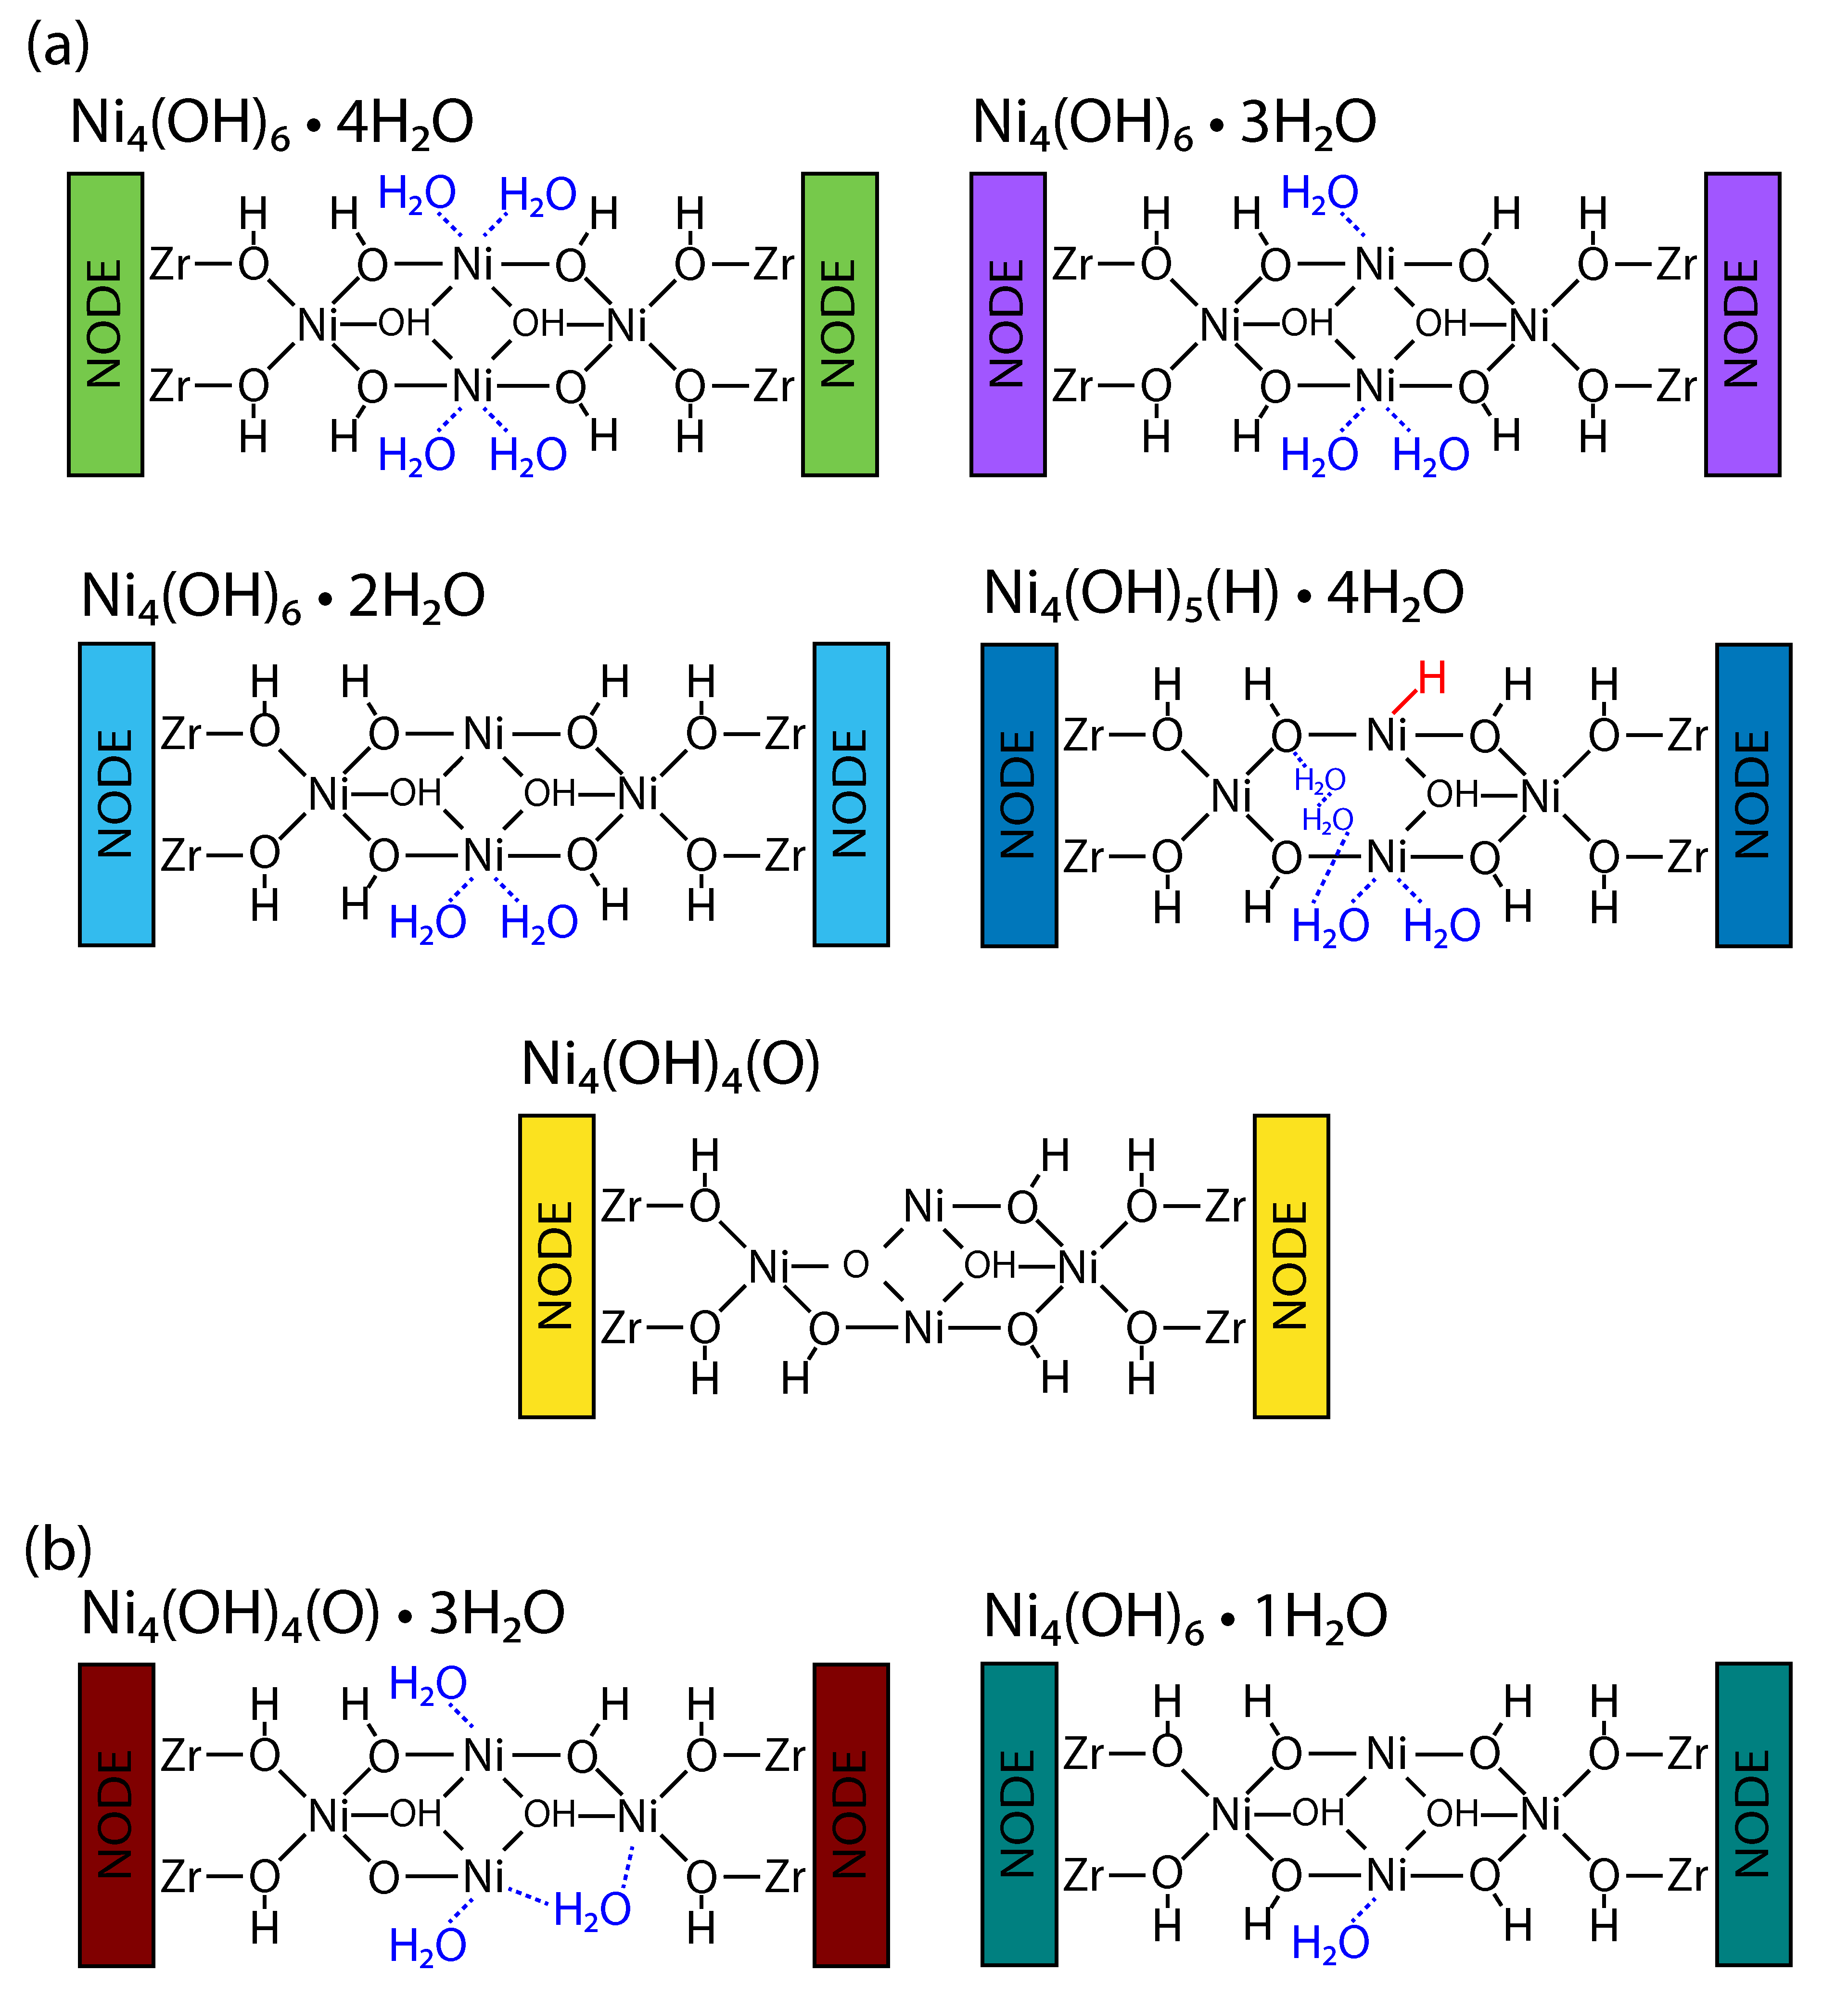
\includegraphics[width=0.75\textwidth]{zi-images/01-Ni-Graphics/2021-MAIN-structure-diagram.png}
    \caption{
    Depictions of (a) structures from Figure~\ref{fig:phase_diagram_Ni} with \ce{Ni-O} coordination numbers $\ge$ 4 and (b) the structure that exhibits a d-PDF that gives the best agreement with that of the synthesized structure. The color scheme is the same as in Figures~\ref{fig:dPDFs-graphic} and \ref{fig:phase_diagram_Ni}. \ce{H2O} molecules and ligands are indicated with blue text, and \ce{Ni} hydrides are indicated with red text for emphasis. 
    }
    \label{fig:Ni-structure-diagram}
\end{figure}

To compare with experiment, d-PDFs for all structures on the phase diagram with \ce{Ni-O} coordination numbers $\ge$ 4 are shown in Figure~\ref{fig:dPDFs-graphic}b. We seek structures that give good agreement with the \ce{Ni-O} and \ce{Ni{\Compactcdots}Ni} peaks seen in the experimental d-PDF, as we find these peaks may be related to structural phenomena that, at present, aren't fully incorporated into any molecular models. \ce{Ni-O} peaks in general agree well with experiment, except for \ce{Ni4(OH)5(H).4H2O} (blue), which exhibits asymmetric split peaks instead of a single peak. From Figure~\ref{fig:Ni-structure-diagram}, this asymmetry is likely caused by an asymmetric ligand environment (Figure~\ref{fig:Ni-MOF-structures}b). Specifically, in addition to \ce{OH} and \ce{H2O} ligands, the \ce{Ni4(OH)5(H).4H2O} (blue) structure comprises a Ni hydride (\ce{H} ligand) as well as a bridge of \ce{H2O} molecules that connect one \ce{Ni} ion with a \ce{OH} ligand on the opposite side of the cluster. That asymmetry in the \ce{Ni-O} peak is not observed experimentally indicates that the ligand environments on the different \ce{Ni} ions in the synthesized structure are more similar than those in structure \ce{Ni4(OH)5(H).4H2O} (blue).  

There is less agreement between simulations and experiments for the \ce{Ni{\Compactcdots}Ni} peaks in the d-PDFs in Figure~\ref{fig:dPDFs-graphic}. In the experimental d-PDF, these peaks are split, suggesting that there is at least some asymmetry in the cluster; however, most of the simulated structures exhibit a single \ce{Ni{\Compactcdots}Ni} peak. The two exceptions are \ce{Ni4(OH)5(H).4H2O} (blue) and \ce{Ni4(OH)4(O)} (yellow), which are shown in Figure~\ref{fig:Ni-MOF-structures}b and c respectively. While \ce{Ni4(OH)5(H).4H2O} (blue) exhibits a highly asymmetric ligand environment including a \ce{H2O} molecule chain and a \ce{Ni} hydride, \ce{Ni4(OH)4(O)} (yellow) comprises mainly \ce{OH} ligands and one \ce{O} ligand (but no \ce{H2O} or \ce{H} ligands). Taken together, these comparisons suggest that the synthesized catalyst exhibits a mix of \ce{OH}, \ce{H2O}, and \ce{O} ligands.

In order to provide further molecular-level insight into the ligand environment of Ni-NU-1000, we generated d-PDFs for the remaining structures in the database (i.e., for the remaining structures not included in Figure~\ref{fig:phase_diagram_Ni}). The structure that gives the best agreement with experiment is \ce{Ni4(OH)4)(O).3H2O} (maroon), which is depicted in Figures~\ref{fig:Ni-MOF-structures}d and \ref{fig:Ni-structure-diagram}b. The d-PDF for this structure is given in Figure~\ref{fig:dPDFs-graphic}c. The \ce{Ni4(OH)4)(O).3H2O} (maroon) structure exhibits a single \ce{Ni-O} peak that is somewhat broader than the for the synthesized structure. It also exhibits split \ce{Ni{\Compactcdots}Ni} peaks like the synthesized structure, although their intensities are somewhat different. The \ce{Ni4(OH)4)(O).3H2O} (maroon) structure exhibits a \ce{Ni-O} coordination number of 5.0 and a mixture of \ce{OH}, \ce{H2O}, and \ce{O} ligands. The ligand environment is asymmetric, leading to split \ce{Ni{\Compactcdots}Ni} peaks at distances in agreement with those observed experimentally. Though this structure is not a thermodynamic minimum according to \textit{ab initio} thermodynamic analysis, we find it competes with the phase space of \ce{Ni4(OH)6.2H2O} (cyan) structure on Figure~\ref{fig:phase_diagram_Ni}; the \ce{Ni4(OH)4)(O).3H2O} (maroon) structure is ~358 kJ/mol of \ce{Ni4(OH)6.2H2O} (cyan) structure.

The last remaining feature of the d-PDFs not yet explored in this work is the \ce{Ni{\Compactcdots}Zr} peak. As for the \ce{Ni{\Compactcdots}Ni} peak, the synthesized structure exhibits split peaks whereas most of the simulated structures exhibit a single peak. The exceptions are the \ce{Ni4(OH)6.4H2O} (green) and \ce{Ni4(OH)4)(O).3H2O} (maroon) structures. While the \ce{Ni4(OH)4)(O).3H2O} (maroon) structure has an asymmetric ligand environment and hence split peaks for distances involving \ce{Ni} are expected, the \ce{Ni4(OH)6.4H2O} (green) structure is highly symmetric. Hence, the split \ce{Ni{\Compactcdots}Zr} peaks may not be caused entirely by asymmetry. Alternatively, the split peaks could be caused by unit cell asymmetry caused by node distortions, which has been previously observed for NU-1000 during \ce{Ni} deposition using AIM and under conditions relevant for catalytic hydrogenation.\cite{PlateroPrats2016} Alternatively the split peaks may arise due to different ligand environments on the \ce{Zr} ions, which we have not explored computationally.

Interestingly, only one structure comprising a \ce{Ni} hydride, i.e., structure \ce{Ni4(OH)5(H).4H2O} (blue), appears on the phase diagram. While this structure exhibits some characteristics in agreement with the synthesized structure, including split \ce{Ni{\Compactcdots}Ni} and \ce{Ni{\Compactcdots}Zr} peaks, it also exhibits split \ce{Ni-O} peaks, which is not observed experimentally, likely due to the significantly different ligand environment created by the hydride itself. These results suggest that the synthesized structure does not include a hydride. This could mean that the active site for hydrogenation catalysis is not a hydride, but rather a \ce{Ni} ion comprising \ce{OH} and/or \ce{H2O} ligands. Alternatively, it could mean that a small fraction (small enough so as to not dominate d-PDF results) of \ce{Ni} clusters within the NU-1000 structure comprise hydrides, and that it is these clusters that are active for hydrogenation catalysis. Further simulations and experiments are needed to clarify these details. 

\section{Conclusions}
%%%%%%%%%%%%%%%%%%%%%%%%%%%%%%%%%%%%%%%%%%%%%%%%%%%%%%%%%%%%%%%%%%%%%
%% Conclusions  
%%%%%%%%%%%%%%%%%%%%%%%%%%%%%%%%%%%%%%%%%%%%%%%%%%%%%%%%%%%%%%%%%%%%%

The rich structural landscape of a \ce{Ni} cluster is modeled using a combination of d-PDF analysis and \textit{ab initio} thermodynamic analysis. We quantify the local structures from modeling using d-PDF analysis, and compare our model structures to experimental d-PDF for a Ni-NU-1000 exposed to \ce{H2} gas. Comparisons with experiments reveal the importance of a high \ce{Ni} coordination environment, which is maintained by coordinated \ce{O}, \ce{OH}, and \ce{H2O} groups to the \ce{Ni} ions of the cluster. A general trend is that the structures containing more \ce{OH} and \ce{H2O} groups show better agreement to the experimental d-PDF in d-PDF analysis, with these structures generally appearing on the phase diagram at large \ce{H2O} chemical potentials. This suggests that there is a sufficient \ce{H2O} chemical potential with Ni-NU-1000, which we are unable to define given that \ce{H2O} is not thought of being present within the system. Further, we identify structures with high \ce{Ni-O} coordination and structural diversity (different \ce{O}, \ce{OH}, and \ce{H2O} ligands). The diverse ligand environment enables asymmetries in the interatomic distances, which enables asymmetries in the \ce{Ni{\Compactcdots}Ni} peaks. Model d-PDFs showing the best agreement with the experimental d-PDFs feature high coordination and a diverse \ce{Ni-O} coordination environment. Given the diverse structures of the \ce{Ni} cluster, our findings suggest that alternate ligand coordination environments should be considered when modeling SSHCs supported on MOFs. 


\section{References}

%The class makes various changes to the way that references are
%handled.  The class loads \textsf{natbib}, and also the
%appropriate bibliography style.  References can be made using
%the normal method; the citation should be placed before any
%punctuation, as the class will move it if using a superscript
%citation style
%\cite{Mena2000,Abernethy2003,Friedman-Hill2003,EuropeanCommission2008}.
%The use of \textsf{natbib} allows the use of the various citation
%commands of that package: \citeauthor{Abernethy2003} have shown
%something, in \citeyear{Cotton1999}, or as given by
%Ref.~\citenum{Mena2000}.  Long lists of authors will be
%automatically truncated in most article formats, but not in
%supplementary information or reviews \cite{Pople2003}. If you
%encounter problems with the citation macros, please check that
%your copy of \textsf{natbib} is up to date. The demonstration
%database file \texttt{achemso-demo.bib} shows how to complete
%entries correctly. Notice that ``\latin{et al.}'' is auto-formatted
%using the \texttt{\textbackslash latin} command.

%Multiple citations to be combined into a list can be %given as
%a single citation.  This uses the \textsf{mciteplus} %package
%\cite{Johnson1972,*Arduengo1992,*Eisenstein2005,*Arduengo%1994}.
%Citations other than the first of the list should be %indicated
%with a star. If the \textsf{mciteplus} package is not %installed,
%the standard bibliography tools will still work but %starred
%references will be ignored. Individual references can be %referred
%to using \texttt{\textbackslash mciteSubRef}:
%``ref.~\mciteSubRef{Eisenstein2005}''.

%The class also handles notes to be added to the bibliography.  These
%should be given in place in the document \bibnote{This is a note.
%The text will be moved the the references section.  The title of the
%section will change to ``Notes and References''.}.  As with
%citations, the text should be placed before punctuation.  A note is
%also generated if a citation has an optional note.  This assumes that
%the whole work has already been cited: odd numbering will result if
%this is not the case \cite[p.~1]{Cotton1999}.

%%%%%%%%%%%%%%%%%%%%%%%%%%%%%%%%%%%%%%%%%%%%%%%%%%%%%%%%%%%%%%%%%%%%%
%% The "Acknowledgement" section can be given in all manuscript
%% classes.  This should be given within the "acknowledgement"
%% environment, which will make the correct section or running title.
%%%%%%%%%%%%%%%%%%%%%%%%%%%%%%%%%%%%%%%%%%%%%%%%%%%%%%%%%%%%%%%%%%%%%
%\begin{acknowledgement}
%
%\hl{authors would like to thank \hl{\ldots}''.
%
%The author thanks Mats Dahlgren for version one of \textsf{achemso},
%and Donald Arseneau for the code taken from \textsf{cite} to move
%citations after punctuation. Many users have provided feedback on the
%class, which is reflected in all of the different demonstrations
%shown in this document.}
%
%\end{acknowledgement}

%%%%%%%%%%%%%%%%%%%%%%%%%%%%%%%%%%%%%%%%%%%%%%%%%%%%%%%%%%%%%%%%%%%%%
%% The same is true for Supporting Information, which should use the
%% suppinfo environment.
%%%%%%%%%%%%%%%%%%%%%%%%%%%%%%%%%%%%%%%%%%%%%%%%%%%%%%%%%%%%%%%%%%%%%
%\begin{suppinfo}
%
%\hl{This will usually read something like: ``Experimental procedures and
%characterization data for all new compounds. The class will
%automatically add a sentence pointing to the information on-line:}
%
%\end{suppinfo}

%%%%%%%%%%%%%%%%%%%%%%%%%%%%%%%%%%%%%%%%%%%%%%%%%%%%%%%%%%%%%%%%%%%%%
%% The appropriate \bibliography command should be placed here.
%% Notice that the class file automatically sets \bibliographystyle
%% and also names the section correctly.
%%%%%%%%%%%%%%%%%%%%%%%%%%%%%%%%%%%%%%%%%%%%%%%%%%%%%%%%%%%%%%%%%%%%%
\bibliography{achemso-demo}

\end{document}